\documentclass{beamer}

% uncomment to generate printer friendly scaled version
\usepackage{pgfpages}
\usepackage[utf8]{inputenc}
\usepackage[ngerman]{babel}
\usepackage[T1]{fontenc}
\usepackage{graphicx}

%listings
\usepackage{listings}
\lstset{numbers=left, numberstyle=\tiny, numbersep=2pt, showstringspaces=false, basicstyle=\scriptsize}
\lstset{language=Java} 

\usetheme{Darmstadt} % default theme
% BUILD SCRIPT HOOKS - DO NOT REMOVE THIS COMMENTS %
%%%%%THEME_PLACEHOLDER_JENKINSBUILD%%%%%
%%%%%HANDOUT_PLACEHOLDER_JENKINSBUILD%%%%%
% END OF BUILD SCRIPT HOOKS %
%\pgfpagesuselayout{4 on 1}[a4paper,border shrink=5mm,landscape]

\setbeamercovered{transparent}
%\setbeamertemplate{footline}[frame number]

\title{Test-driven development}
\subtitle{mit JUnit, Mockito und PowerMock}

\institute[TD 2k11]{Computerseminar Tondorf 2011}

\author[F. Becker, B. Neff]{
        Felix Becker \&
	Benjamin Neff
}

\begin{document}

	\begin{frame}
		\titlepage
	\end{frame}

	\begin{frame}
		\frametitle{Agenda}
		\setcounter{tocdepth}{1}
		\tableofcontents
	\end{frame}
	
	%
	% Einfuehrung
	%

	\logo{}
	\section{Einführung}
	
		\subsection{Einführung in Test-driven development}

			\begin{frame}
				\frametitle{Was ist Unit-Testing?}

				Unit-Testing:
				\begin{itemize}
					\item{Test einzelner Komponente (Unit)}
					\item{Komponente während des Tests vom Gesamtsystem isoliert (Seiteneffekte vermeiden)}
					\item{Test deckt Normalverhalten und explizit auch den Fehlerfall ab}
				\end{itemize}
				\pause
				Ziele von Unit-Testing:
				\begin{itemize}
					\item{Frühzeitiges Erkennen von Fehlern}
					\item{Test von spezifiziertem Komponentenverhalten (Refactoring!)}
					\item[]{\color{red}\textbf{$\Rightarrow$ Wartbarkeit und hohe Qualität}}
				\end{itemize}
				
			\end{frame}

			\begin{frame}
				\frametitle{Was ist Test-driven development?}
				
				TDD:
				\begin{itemize}
					\item{Entwicklungstechnik aus dem Bereich der agilen Softwareentwicklung}
					\item{Erst Testcases, dann Implementierung der Komponente}
					\item{Testcases sind Black/Grey-Box Tests}
					% Beispiel für Grey-Box: Komponente die Socket aufmacht. Socket explizit killen.
				\end{itemize}
				\pause
				Ziele von TDD:
				\begin{itemize}
					\item{Klar definiertes Komponentenverhalten zum Implementierungszeitpunkt}
					\item{Sicherstellung der Testabdeckung} % Wer schreibt nacher schon noch Testcases? Zeitdruck / Faulheit..
					\item{Sicherstellung der Testqualität (Kein Whiteboxtest!)} % kein test der internen komponentenimplementierung!
					\item[]{\color{red}\textbf{$\Rightarrow$ Wartbarkeit und hohe Qualität}}
				\end{itemize}
			\end{frame}

	%
	% Tools und Frameworks
	%
	
	\section{Tools \& Frameworks}

		\subsection{Was gibt es für Tools und Frameworks?}

			\begin{frame}
				\frametitle{Frameworks}

				\begin{itemize}
					\item{JUnit}
					\item{Mockito}
					\item{PowerMock}
					\item{(TestNG)}
				\end{itemize}
			\end{frame}

			\begin{frame}
				\frametitle{Continuous Integration}

				\begin{itemize}
					\item{Hudson / Jenkins}
					\item{Continuum}
					\item{CruiseControl}
					\item{\ldots}
				\end{itemize}
			\end{frame}

			\begin{frame}
				\frametitle{EMMA}

				\begin{figure}[htb]
					\begin{center}
						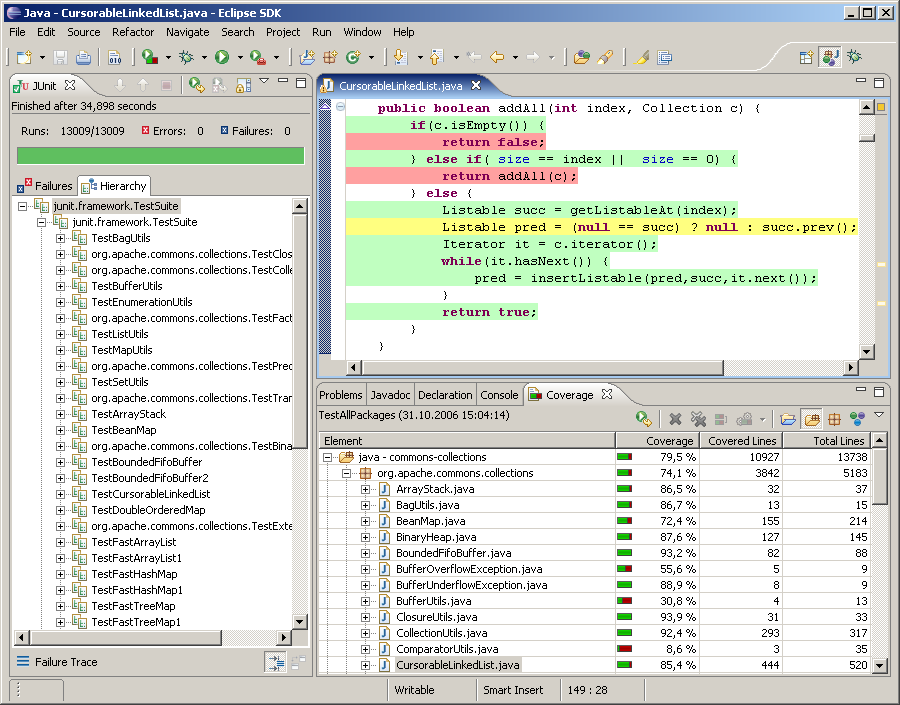
\includegraphics[scale=0.25]{images/eclemma}
					\end{center}
					\caption{http://www.eclemma.org/images/screen.png}
				\end{figure}
			\end{frame}

	%
	% JUnit und Mockito
	%
	
	\section{JUnit \& Mockito}

		\logo{
\includegraphics[height=1cm]{images/junit}}
		\subsection{Testen mit JUnit}

			\begin{frame}
				\frametitle{Was ist JUnit?}

				\begin{itemize}
					\item{''Standard''-Framework für Java-Unittests}
					\item{Testergebnis OK (grün) / nicht OK (rot)}
					\item{Sehr einfache Bedienung (Annotations, \ldots)}
					\item{Aktuelle Version: JUnit 4}
				\end{itemize}
			\end{frame}

			\begin{frame}[fragile]
				\frametitle{Test-Klasse: Int-Calculator}

				\begin{lstlisting}
					public class CalculatorTest {
					  private Calculator calculator;

					  @Before
					  public void setup() {
					    calculator = new Calculator();
					  }

					  @Test
					  public void testSum(){
					    assertEquals(5, calculator.sum(2, 3));
					  }

					  @Test
					  public void testSumWithNegativeValue(){
					    assertEquals(-5, calculator.sum(-2, -3));
					  }
					  // ...
					}
				\end{lstlisting}
			\end{frame}
		
			\begin{frame}[fragile]
				\frametitle{Int-Calculator}

				\begin{lstlisting}
					public class Calculator {
					  public int sum(int x, int y){
					    return x + y;
					  }

					  public int divide(int x, int y){
					    return x / y;
					  }
					  // ...
					}
				\end{lstlisting}
			\end{frame}

			\begin{frame}[fragile]
				\frametitle{Fehlerfall testen}

				\begin{lstlisting}
					@Test(expected = ArithmeticException.class)
					public void expectExceptionOnDivisionByZero(){
					  calculator.divide(1, 0);
					}
				\end{lstlisting}
			\end{frame}

			\begin{frame}
				\frametitle{Die Klasse org.junit.Assert und Annotations}

				\begin{block}{Assertions}
					assertArrayEquals, assertEquals, assertFalse, assertNotNull, assertNotSame, assertNull, assertSame, assertThat, assertTrue, fail
				\end{block}
				\begin{block}{Annotations}
					After, AfterClass, Before, BeforeClass, Ignore, Test, RunWith
				\end{block}
			\end{frame}

		\logo{
\includegraphics[height=1cm]{images/mockito}}
		\subsection{Mocking mit Mockito}

			\begin{frame}
				\frametitle{Was ist ein Mock?}

				\begin{itemize}
					\item{engl. Mock-up (Attrappe / Simulation)}
					\item{Attrappe eines Objekts}
					\item{Selbe Schnittstelle wie das Original-Objekt}
					\item{Ersatz für Komponenten, die die zu testende Komponente benötigt}
					\item{Garantiert definiertes Verhalten während des Tests}
				\end{itemize}
			\end{frame}

			\begin{frame}
				\frametitle{Mockito}

				\begin{itemize}
					\item{Sehr einfache Mock-Erstellung}
					\item{Mockverhalten leicht konfigurierbar}
					\item{Aufzeichnung aller Mock-Calls}
					\item{Werkzeuge zur Verifikation von Mock-Calls}
				\end{itemize}
			\end{frame}

			\begin{frame}[fragile]
				\frametitle{Mockito Beispiel}

				\begin{lstlisting}
					CokeRepository cokeRepo = mock(CokeRepository.class);
					FantaRepository fantaRepo = mock(FantaRepository.class);

					when(cokeRepo.get("afri")).thenReturn(new AfriCola());
					when(fantaRepo.get(anyString())).thenThrow(new EmptyException());

					DrinksDispenser drinkDispenser = new DrinksDispenser();
					drinkDispenser.setCokeRepository(cokeRepo);
					drinkDispenser.setFantaRepository(fantaRepo);

					assertTrue(drinkDispenser.getAfri() instanceof AfriCola);
					assertNull(drinkDispenser.getFanta());

					verify(cokeRepo, times(1)).get("afri");
					verify(fantaRepo, times(1)).get(anyString());

					verifyNoMoreInteractions(cokeRepo);
					verifyNoMoreInteractions(fantaRepo);
				\end{lstlisting}
			\end{frame}

			\begin{frame}[fragile]
				\frametitle{Spying}

				\color{red}\textbf{Code smell!}
				\color{black}
				\begin{lstlisting}
					@Test
					public void setSize() {
					  template = Mockito.spy(template);

					  template.setSize(23, 42);

					  verify(template).setPreferredSize(new Dimension(23, 42));

					  Assert.assertEquals(23, template.getWidth());
					  Assert.assertEquals(42, template.getHeight());
					}
				\end{lstlisting}
			\end{frame}

			\begin{frame}
				\frametitle{Die Klasse org.mockito.Mockito}

				\begin{block}{Verifications}
					verify, verifyNoMoreInteractions, verifyZeroInteractions
				\end{block}

				\begin{block}{VerificationModes}
					atLeast, atLeastOnce, atMost, never, only, times
				\end{block}
			\end{frame}

			\begin{frame}
				\frametitle{Die Klasse org.mockito.Matchers}

				\begin{block}{Matcher}
					any, anyBoolean, anyByte, anyChar, anyCollection, anyCollectionOf, anyDouble, anyFloat, anyInt, anyList, anyListOf, anyLong, anyMap, anyObject, anySet, anySetOf, anyShort, anyString, anyVararg, argThat, booleanThat, byteThat, charThat, contains, doubleThat, endsWith, eq, floatThat, intThat, isA, isNotNull, isNull, longThat, matches, notNull, refEq, same, shortThat, startsWith
				\end{block}
			\end{frame}
		%\subsection{Partial Mocking} frame wenn es eine mockito technologie ist

	%
	% PowerMock
	%
	
	\logo{
\includegraphics[height=1cm]{images/powermock}}
	\section{PowerMock}

		\subsection{Einleitung}

			\begin{frame}
				\frametitle{PowerMock}

				\begin{itemize}
					\item{Mit Java-Bordmitteln normalerweise nicht mockbare Komponenten mocken}
					\item{Deep and dark magic}
						\begin{itemize}
							\item{Byte code Manipulation (javaassist)}
							\item{Classloader-Manipulation}
						\end{itemize}
				\end{itemize}
			\end{frame}

		\subsection{Constructor call prevention}

			\begin{frame}[fragile]
				\frametitle{A constructor nightmare}

				\begin{lstlisting}
					public class Foo {
					  public Foo(){
					    if(!MyFrameworkMegaUtil.isFrameworkProperlyInitialized()){
					      MyFrameworkMegaUtil.initializeFramework();	
					    }
					  }

					  public int sum(int x, int y){
					    return x+y;
					  }
					}
				\end{lstlisting}
			\end{frame}

			\begin{frame}[fragile]
				\frametitle{Solution!}

				\begin{lstlisting}
					public class FooTest {
					  @Test
					  public void testSum(){
					    Foo comp = WhiteBox.newInstance(Foo.class);
					    assertEquals(5, comp.sum(2, 3));
					  }
					}
				\end{lstlisting}
			\end{frame}

			\begin{frame}[fragile]
				\frametitle{Problem mit Socket}

				\begin{lstlisting}
					public class Connection {
					  private Socket socket;

					  public void connect() throws UnknownHostException,
					      IOException {
					    socket = new Socket("localhost", 1337);
					  }

					  public void disconnect() throws IOException {
					    socket.close();
					  }

					  // ...
					}
				\end{lstlisting}
			\end{frame}

			\begin{frame}[fragile]
				\frametitle{Solution!}

				\begin{lstlisting}
					@PrepareForTest(Connection.class)
					@RunWith(PowerMockRunner.class)
					public class ConnectionTest {
					  @Test
					  public void testConnectAndDisconnect() throws Exception {
					    final Socket socket = mock(Socket.class);

					    PowerMockito.whenNew(Socket.class)
					      .withArguments(anyString(), anyInt())
					      .thenReturn(socket);

					    final Connection connection = new Connection();
					    connection.connect();
					    connection.disconnect();

					    PowerMockito.verifyNew(Socket.class)
					      .withArguments("localhost", 1337);
					    verify(socket).close();
					  }
					}
				\end{lstlisting}
			\end{frame}

		\subsection{Static / Final Mocks}

			\begin{frame}[fragile]
				\frametitle{A static nightmare}

				\begin{lstlisting}
					public class Foo {
					  public int testStatic(){
					    int sth = sth();
					    int y = DrEvil.getEvil(sth);	
					    return sth + y;
					  }
					  // ...
					}

					public class DrEvil {
					  public static int getEvil(int x){
					    return doReallyEvilStuff();
					  }
					}
				\end{lstlisting}
			\end{frame}

			\begin{frame}[fragile]
				\frametitle{Solution!}

				\begin{lstlisting}
					@PrepareForTest(DrEvil.class)
					@RunWith(PowerMockRunner.class)
					public class FooTest {
					  @Test
					  public void testStatic(){
					    PowerMockito.mockStatic(DrEvil.class);
					    Mockito.when(DrEvil.getEvil(anyInt())).thenReturn(1);
					    Foo foo = new Foo();
					    assertEquals(1,foo.testStatic());

					    // static verification
					    PowerMockito.verifyStatic();
					    DrEvil.getEvil(anyInt());
					  }
					}
				\end{lstlisting}
			\end{frame}

			\begin{frame}[fragile]
				\frametitle{A final nightmare}

				\begin{lstlisting}
					public class Foo {
					  private MyCoolLibrary lib;

					  public void setLib(final MyCoolLibrary lib) {
					    this.lib = lib;
					  }

					  public void testFinal() {
					    lib.doFinal();
					    // ...
					  }
					  // ...
					}

					public final class MyCoolLibrary {
					  public void doFinal() {
					    // ...
					  }
					}
				\end{lstlisting}
			\end{frame}

			\begin{frame}[fragile]
				\frametitle{Solution!}

				\begin{lstlisting}
					@PrepareForTest(MyCoolLibrary.class)
					@RunWith(PowerMockRunner.class)
					public class FooTest {
					  @Test
					  public void testFinal() {
					    final MyCoolLibrary lib = mock(MyCoolLibrary.class);

					    final Foo foo = new Foo();
					    foo.setLib(lib);
					    foo.testFinal();

					    verify(lib).doFinal();
					  }
					}
				\end{lstlisting}
			\end{frame}

	%
	% Abschluss 
	%

	\logo{}
	\section{Abschluss}

		\subsection{Common Pitfalls}

			\begin{frame}
				\frametitle{Beachten!}

				\begin{itemize}
					\item{Nicht die Implementierung sondern das Verhalten der Komponente testen (Refactoring von ungetestetem Code!)}
					\pause
					\item{Zu viele static-Mocks weisen auf Design-Probleme hin}
					\pause
					\item{Zu niedrige Code-Coverage nach Testfertigstellung weist auf ein Design-Problem hin (auch Boilerplate abdecken!)}
					\pause
					\item{Immer Fehlerfallverhalten der Komponente testen (Logging, Returnvalues, Exceptions, \ldots)}
					\pause
					\item{Zu ''lange'' Testfälle weisen auf ein Problem hin}
				\end{itemize}
			\end{frame}

		
		\subsection{Danke und Quellen}

			\begin{frame}
				Fragen? Nein? Danke!
			\end{frame}

			\begin{frame}
				\frametitle{Quellen und Wissenswertes}

				\scriptsize
				Wissenswertes
				\begin{itemize}
					\item{\url{http://de.wikipedia.org/wiki/Modultest}}
					\item{\url{http://de.wikipedia.org/wiki/Testgetriebene\_Entwicklung}}
					\item{\url{http://de.wikipedia.org/wiki/Mock-Objekt}}
				\end{itemize}

				JUnit \& Mockito \& PowerMock
				\begin{itemize}
					\item{JUnit: \url{http://www.junit.org}}
					\item{Mockito: \url{http://www.mockito.org}}
					\item{PowerMock: \url{http://code.google.com/p/powermock/}}
				\end{itemize}

				Hudson \& Jenkins \& EMMA
				\begin{itemize}
					\item{Hudson: \url{http://www.hudson-ci.org}}
					\item{Jenkins: \url{http://www.jenkins-ci.org}}
					\item{EMMA: \url{http://emma.sourceforge.net}}
					\item{Ecl-Emma: \url{http://www.eclemma.org}}
				\end{itemize}
			\end{frame}

\end{document}
